\comm{
\subsubsection{LISA Baseline model Limitation}

Prediction cost in baseline method consists of following two parts.

\begin{enumerate}
	\item Search cost for the cell which contains the key. This cost will be equal to $log_{2}N_{1}$, where $N_{1}$ is the number of cells into which mapped values are divided.
	
	\item Cost associated with sequentially comparing the query point key value against keys inside the cell found in previous search. On average this cost will be equal to $N_{2}\slash2$, where $N_{2}$ is the number of keys in a cell.   
	
If cell size is large, number of cells will be smaller, number of keys per cell will be higher, resulting in higher cost of sequential scan with in the cell. 
\end{enumerate}
Consider the example in figure \ref{fig:BaseLine_Method_Limitation}. Dataset is divided into 3 sections based on the mapped values. Any point or range query in the second triangle(page) will result into a sequential scan through all 9 keys in the cells.

\begin{figure*}[t]
    \centering
    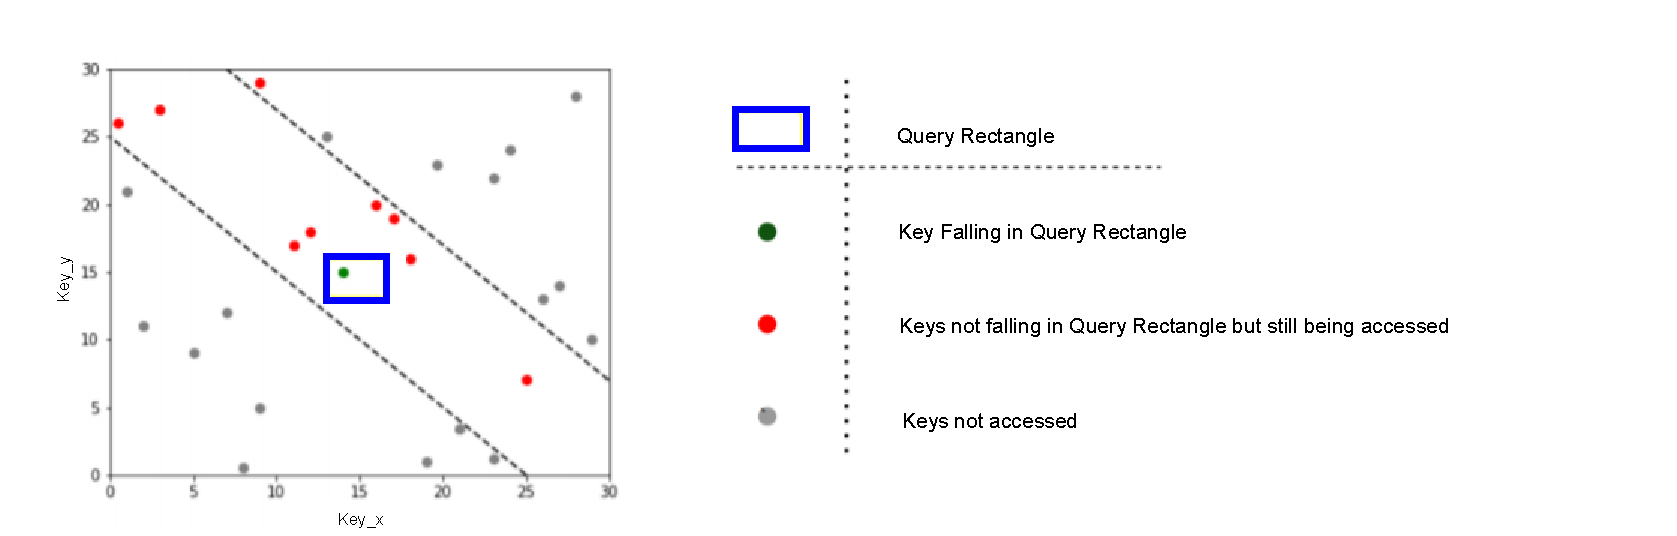
\includegraphics[width=1.3\textwidth]{graphs/Baseline_limitation.pdf}
    \caption{Baseline Method Limitation }
    \label{fig:BaseLine_Method_Limitation}
\end{figure*}
}


\subsubsection {LISA Baseline model search optimization for smaller values of N}
%In lisa baseline model, we need to linearly search for the query key in a cell. 
In case of high dimensional key values, key with in a cell can not be searched with mapped value, as a large number of keys can have the same mapped value. However for the 2 dimensional scenario, we can get considerable savings in search cost by replacing sequential scan based on keys values to binary search based on mapped value. As in the original method, search process  will consist of two parts.
\begin{enumerate}
	\item Find the cell which contains the query key based on mapped value using binary search. 
	\item With in the cell, replace sequential search based on query key value with the  binary search based on query key mapped value. Once mapped value is found, do a lookup in the neighbourhood of the found key based on query key 2 dimensional value. 
\end{enumerate}
As shown in Fig. \ref{fig:LISA_Baseline_Optimization}, we get significant savings in the query time with this approach for smaller values of N. As the value of $N$ increases, number of Keys per cell decreases, and savings in avoiding sequential search gets normalized. 


\begin{figure}
 \centering
     \begin{subfigure}[b]{0.45\textwidth}
         \centering
         \begin{tikzpicture}[font=\small]
	\pgfplotsset{compat=1.10, width=\textwidth, height=\textwidth,every axis
	legend/.append style={
		at={(1,1)},
		anchor=north east}}
	\begin{axis}[
		xmode=log,
		xlabel=$N$,
		ylabel=Average Query Time (ms),
		xtick={10,100,1000,10000},
		legend style={nodes={scale=0.55, transform shape}}
	]
	\addplot[smooth, mark=x, blue]
	coordinates{
		(10, 46.7173)
		(100, 4.8086)
		(1000, 0.7271)
		(10000,0.3301)
		%(100000,0.2381)
	};
	\addplot[smooth,mark=o,red]
  	coordinates{
        (10, 0.2855)
		(100,0.2823)
		(1000, 0.2806)
		(10000,0.2794)
		%(100000,0.2322)
	};
  
    %\legend{LISA Baseline, LISA Baseline Optimized}
	\end{axis}
\end{tikzpicture}
         \caption{Training Size 100K}
         \label{fig:2d_exp4_3_1}
     \end{subfigure}
     \begin{subfigure}[b]{0.45\textwidth}
         \centering
         \begin{tikzpicture}[font=\small]
	\pgfplotsset{compat=1.10, width=\textwidth, height=\textwidth,every axis
	legend/.append style={
		at={(1,1)},
		anchor=north east}}
	\begin{axis}[
		xmode=log,
		xlabel=$N$,
		ylabel=Average Query Time (ms),
		xtick={10,100,1000,10000},
		legend style={nodes={scale=0.75, transform shape}},
		scaled y ticks = base 10:-2,
	]
	\addplot[smooth, mark=x, blue]
	coordinates{
		(10, 347.5613)
		(100, 40.1451)
		(1000, 4.4732)
		(10000,0.6697)
		%(100000,0.2944)
	};
	\addplot[smooth,mark=o,red]
  	coordinates{
        (10, 0.2905)
		(100,0.2858)
		(1000, 0.2844)
		(10000,0.2831)
		%(100000,0.2322)
	};
  
    \legend{LISA Baseline, LISA Baseline Optimized}
	\end{axis}
\end{tikzpicture}
         \caption{Training Size 1M}
         \label{fig:2d_exp4_3_2}
     \end{subfigure}
     \caption{Point query results comparison between LISA Baseline and Optimized Model for different training sizes.}
     \label{fig:LISA_Baseline_Optimization}
\end{figure}

